\documentclass[12pt]{article}
\usepackage[utf8]{inputenc}
\usepackage{csquotes}
\usepackage[ngerman]{babel}
\usepackage[backend=biber, style=apa, sorting=nty]{biblatex}
\renewcommand*{\bibfont}{\small}
\addbibresource{citation.bib}
\usepackage[T1]{fontenc}
\usepackage[top=2cm,left=3cm,right=2cm,bottom=2cm]{geometry}
\usepackage[parfill]{parskip}
\usepackage[font=normalsize]{caption}
\usepackage{hyperref}
\usepackage{multirow}
\usepackage{amsmath}
\usepackage{amssymb}
%% From HAW-Template
\usepackage{setspace}
\usepackage{listings}
\usepackage{graphicx} %% Important for including pictures
\graphicspath{{./images/}}
%% define colors in article
\usepackage{xcolor}
\definecolor{arsenic}{rgb}{0.23, 0.27, 0.29}
\definecolor{smokyblack}{rgb}{0.06, 0.05, 0.03}
\definecolor{coolblack}{rgb}{0.0, 0.18, 0.39}
\definecolor{mistyrose}{rgb}{1.0, 0.89, 0.88}
\hypersetup{
  colorlinks=true,
  linkcolor=black,
  filecolor=cyan,
  urlcolor=coolblack,
  citecolor=black,
}

%% \linespread{1.25} %% Paragraphs 1.5 lineheight
\onehalfspacing

%% \setmainfont{Arial}
\usepackage{uarial}
\renewcommand{\familydefault}{\sfdefault}

%% to set size of headings as normalsize 12pt
\usepackage{sectsty}
\sectionfont{\normalsize}
\subsectionfont{\normalsize}

%% to change space of headings to 0
\usepackage{titlesec}
\titlespacing*{\section}
{0pt}{12pt}{6pt}
\titlespacing*{\subsection}
{0pt}{6pt}{6pt}
\titlespacing*{\subsubsection}
{0pt}{6pt}{6pt}

%% set headers 
\usepackage{fancyhdr}
\pagestyle{fancy}
\fancyhf{}
\rhead{\textit{\footnotesize{Duy Nguyen. 2359864}}}
\rfoot{\thepage}
%% change paragraph margins
\usepackage{changepage}
\usepackage{subcaption}
\title{Vorstellung der Drucksensoren}
\author{Duy Nguyen}

%% Begin document
\begin{document}
\pagestyle{empty}
\color{smokyblack}

\setlength{\parskip}{1ex}
\begin{table}[t]
  \begin{center}
    \begin{tabular}{p{0.7\textwidth}r}
      \small{HAW-Hamburg} & \multirow{4}{*}{
\includegraphics[width=4.6cm]{haw-logo}} \\
      \small{Vorlesung Messtechnik} &  \\
      \small{Sommersemester 2021} & \\
      \small{Prof. Dr. Carsten Frank} & 
    \end{tabular} 
  \end{center}
\end{table}

\vspace{2cm}

\textsf{\textit{\Large{Hausarbeit}}}

\color{arsenic}
\textsf{\textbf{\huge{Feinstaubmessstation, ein Proof of concept Modulaufbau}}}
\setlength{\parskip}{0.8em}
\color{smokyblack}
%% Add abstract paragraph

\begin{adjustwidth}{3em}{0pt}
\begin{flushleft}
	\textit{Duy Nguyen} 

  \vspace{-12pt}

  \textit{\footnotesize{Feinstaubsgruppe: Duy Nguyen, Ferris Fensky, Dennis Dick}}
\end{flushleft}
\end{adjustwidth}

\tableofcontents
\newpage
\listoffigures
\addcontentsline{toc}{section}{Abbildungsverzeichnis}
\listoftables
\addcontentsline{toc}{section}{Tabellenverzeichnis}

%% Uncomment these lines to input manually list of abbreviations as IV from external file
%% \input{abbreviationpage}
%% \addcontentsline{toc}{section}{List of abbreviations}

\newpage
\pagestyle{fancy}
\section{Feinstaubmessstation}
\label{sec:feinstaubmessstation}

Ein "Proof of concept" wird in diesem Abschnitt vorgestellt und bewertet, ob es ein möglich günstig und praktisches Konzept gibt, mit dem man selbst durch Aufbau eines Messgeräts die Feinstaubbelastung in seiner Umgebung beobachten könnte. Idee ist beruhend auf Lichtstreuungsprinzip. Eine Lichtquelle (Laser oder LED) und eine Fotodiode sorgt dafür, dass die Feinstaubpartikeln, die durch eine Messzelle fliehen, erkennbar werden. Folgendes sollten die verfügbare Feinstaubmessgeräte, den theoretischen Aufbau eines Konzeptes mit Bauteilen bzw. Kosten, und eine Schlussfolgerung präsentiert werden.  

\subsection{Verfügbare Feinstaubmessgeräte im Markt}
\begin{figure}[h!]
  \centering
  \label{fig:sds011}
  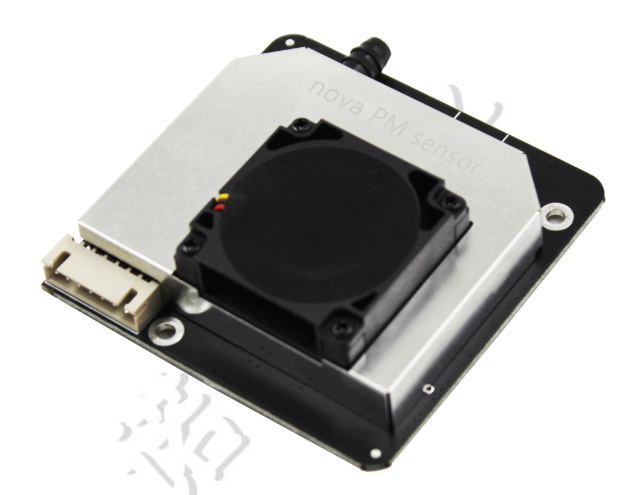
\includegraphics[width=0.4\textwidth]{sds011}
  \caption{Nova Fitness SDS011 Feinstaubmessmodul (\cite{Inovafitness.2020})}
\end{figure}
Seit 2015 stellt Nova Fitness (ein chinesisches Unternehmen von Shandong) die SDS011 - Feinstaubmessmodul her. Damit kann man direkt mit einem Mikrokontroller verbunden und die Messwerte auslesen. Ein Konzept wurde damit von Open Knowledge Foundation Stuttgart aufgebaut, das Projekt heißt Sensor.Community. Gleichzeitig mit Feinstaubmessung vom Modul SDS011, werden Temperatur und Luftfeuchtigkeit durch das Modul DHT22 gemessen, optional werden alle mögliche Sensor z.B SD18B20, BME280 (Luftfeuchtigkeit/-druck Sensor) mit Hilfe vom Mikrokontroller NodeMCU ESP8266 betrieben. Nach der Verbindung mit dem eingestellten Mikrokontroller ist die Messdaten zu einem API geschickt und jeder Zeit aufrufbar. Da sind noch mehrere Studien, die über die Möglichkeit von Aufbau eines kostengünstigen Feinstaubsensor diskutierten. z.B Modul Shinyei PPD42NS (\cite{Austin.2015}, \cite{Holstius.2014}, \cite{Gao.2015} )

\subsection{Theoretischer Aufbau eines Konzeptes zum Feinstaubmessung}

\subsubsection{Feinstaubmessmodul}
Hier wollen wir das SDS011 Modul durch einfaches Konzept ersetzen und ein gesamtes System von Anfang bis Ende aufbauen. Basiert auf Lichtstreuungsprinzip, die Feinstaubmessmodul wird wie in folgende Abbildung vorgestellt.

\begin{figure}[h!]
  \centering
  \label{fig:ftmm}
  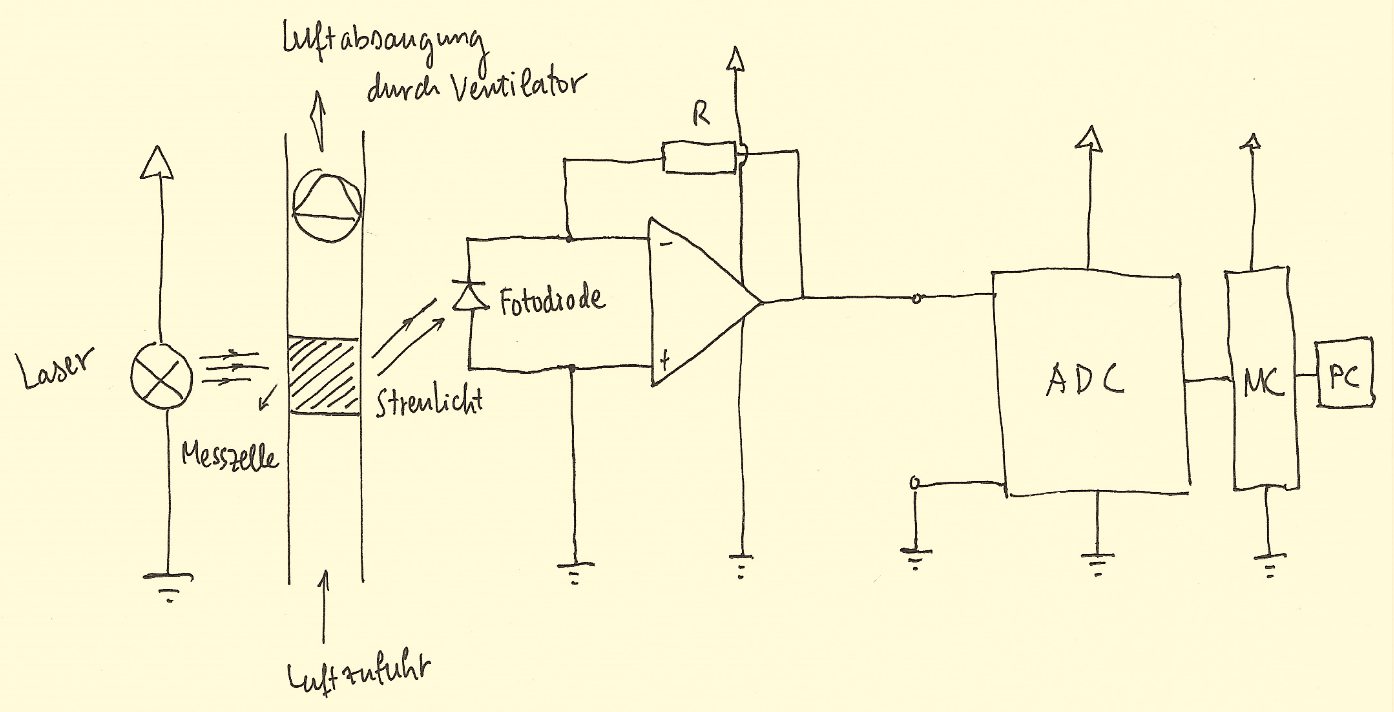
\includegraphics[width=\textwidth]{feinstaubschaltungneu2}
  \caption{Aufbauschema Feinstaubmessmodul}
\end{figure}

\subsubsection{Gesamtes Messstation im Überblick}
\begin{figure}[h!]
  \centering
  \label{fig:gesamtschema}
  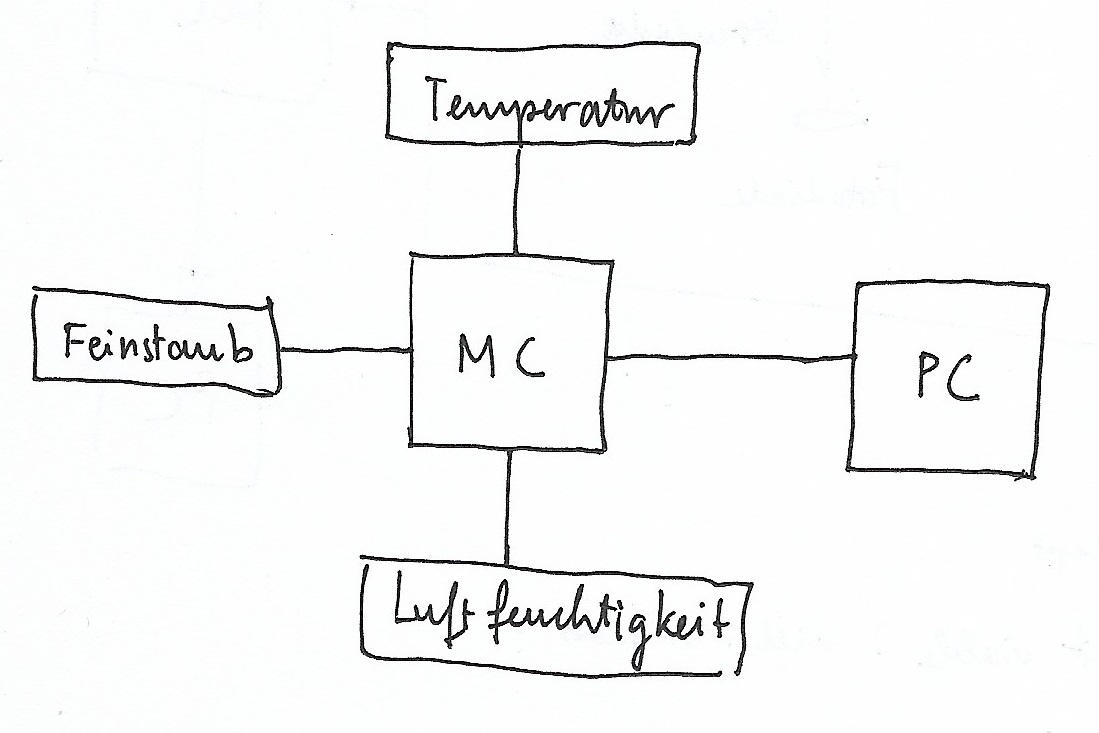
\includegraphics[width=0.6\textwidth]{gesamtschema}
  \caption{Gesamtes Schema der Messstation}
\end{figure}
Wir sollten bei der Messung von Feinstaub mit billigen elektrischen Sensoren auf einige Probleme stoßen, nämlich Feuchtigkeit und Temperatur. Studien zeigen, dass eine hohe Luftfeuchtigkeit die Qualität der Feinstaubmessungen beeinflusst (\cite{BerndLaquai.2017} ). Kleine Wassertröpfchen können eine Menge an Stoffen aufnehmen, die größer sein kann als die Größe der Partikel, die wir messen möchten. Es gibt Lösungen, dass wir die Luftströme vor der Messung aufheizen können, aber das ist für einen billigen kleinen Luftverschmutzungssensor nicht relevant. An dieser Stelle kann ein weiterer Feuchtesensor helfen, der als Koeffizient mitspielen und das Ergebnis korrigieren würde. Das passiert meistens bei regnerischem Wetter, aber an warmen Tagen gibt es auch Probleme mit dem Lichtdetektor in unserem Modul. Diese Fotodiode ist empfindlich bei hohen Temperaturen und verzerrt die Ausgabe. Dieselbe Lösung mit Temperaturkoeffizient kann verwendet werden. Da es mit den Korrekturfaktoren arbeitet, sollten wir das System nicht dort einsetzen, wo extreme Schwankungen auftreten können (wie Wetter im Freien). 

Für dieses Projekt wird der Fotodiode BPX61 gewählt, weil hohe Reaktionsgeschwindikeit gebraucht wird (Einkauf: \cite{Conrad.8312021}, Datenblatt: \cite{OSRAM.2014}). Die Fotodiode hat eine relativ spektrale Empfindlichkeit von 400nm bis 1100nm. Hier können wir viele verschiedene Variablen mit der Lichtreichweite ausprobieren, Laser ist eine gute Option, weil er eine gute Lichtintensität und ein stabiles gerades Licht bei 650nm Wellenlänge hat, aber viele LEDs haben heutzutage auch eine gute Qualität, um die Arbeit zu erledigen, und sie sind in vielen Farben wie Grün erhältlich (550nm Lichtwelle) zB grüne LED. (Einkaufslink: \cite{LEDAma}, Datenblatt: \cite{Alldatasheet.8282021}). Das ist eines der Experimente, die wir machen können, um zu testen, welches Licht die besseren Ergebnisse liefert.

\begin{figure}[h!]
  \centering
  \begin{subfigure}[b]{0.45\linewidth}
    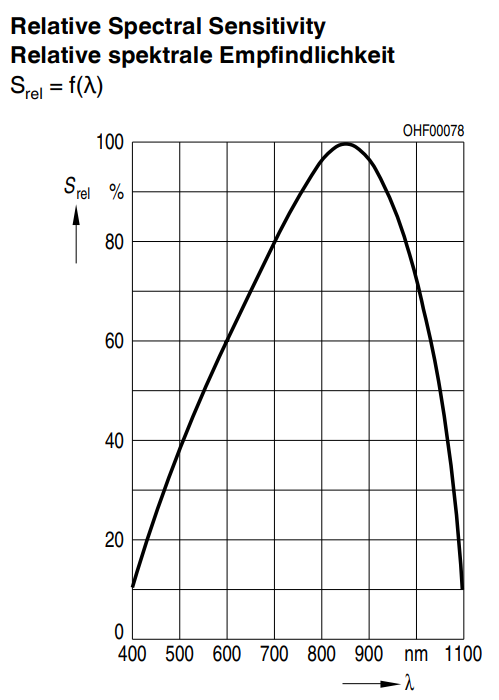
\includegraphics[width=\linewidth]{bpx61empfindlichkeit}
    \caption{BPX61. Spektraler Bereich der Fotoempfindlichkeit (\cite{OSRAM.2014}) }
  \end{subfigure}
  \begin{subfigure}[b]{0.45\linewidth}
    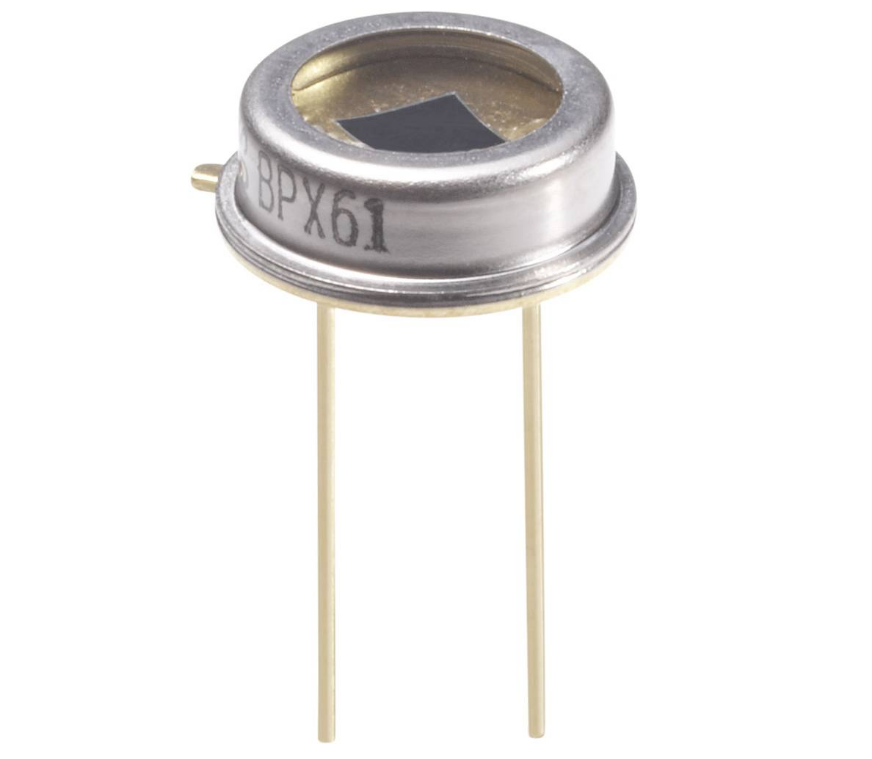
\includegraphics[width=\linewidth]{bpx61}
    \caption{BPX61 Fotodiode (\cite{Conrad.8312021})}
  \end{subfigure}
  \caption{BPX61 Fotodiode mit ihrem spektralen Bereich} 
  \label{fig:bpx61}
\end{figure}

Das Gehäuse von dem Feinstaubmessmodul wird ähnlich wie SDS011 gebaut. 

\begin{figure}[h!]
  \centering
  \label{fig:sds011innen}
  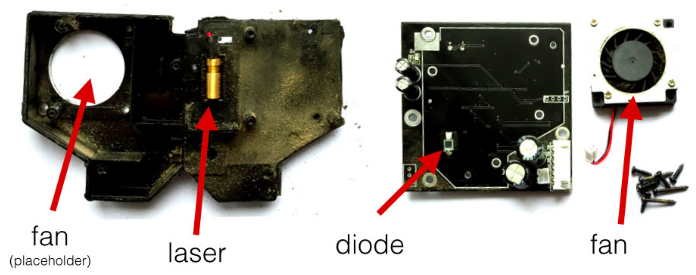
\includegraphics[width=0.5\textwidth]{sds011innen}
  \caption{Innenaufbau von SDS011 (\cite{TheWorldAirQualityIndex.6202021})}
\end{figure}

Für die Temperatur haben wir den PT100-Sensor, der bereits im ersten Abschnitt vorgestellt wird. Ein weiterer zusätzlicher Temperatursensor ist mit dem Feuchtigkeitssensor DHT22 (Einkaufslink: (\cite{DHT22Kaufen}), Datenblatt: (\cite{AZDelivery.2021}) ) eingebaut, der insgesamt als guter Vergleich dienen kann, um die Leistung des PT100-Temperatursensors zu testen. Natürlich ist es nicht notwendig, eine PT100-Schaltung zu bauen, da es komplizierter wird, als wir benötigen (Verstärker INA333, ADC MAX11164 und die Drähte und Widerstände). Nachdem wir alle Sensoren mit ihrer Ausgangsspannung bereits eingestellt haben, sind alle dann mit dem Mikrocontroller NodeMCU ESP8266 verbunden. Der hat ein WLAN-Modul, dass die Daten über eine einfache Netzwerkeinrichtung an unsere API weitergegeben und in Datenbank gespeichert werden können.

\subsection{Schlussfolgerung}
Insgesamt ist dies ein sehr einfaches Konzept, das leicht austauschbare Komponenten hat und nicht schwer zu bauen ist (geschätzte Zeit 2 Stunden). Alle Komponente sind für unseren Temperatursbereich geeignet und nutzen meistens die Spannungsversorgung von 5V (von Laser KY-008 bis zu Mikrokontroller). Bei der Feuchtekompensation ist zu erwähnen, dass das Feinstaubmessmodul bei Regenwetter mit Kondenswasser befüllt werden kann. Das kann behoben werden, wenn wir das Modul gut genug mit Wasserisolierung bauen und die Luftströme von den elektrischen Komponenten getrennt werden müssen. Bei weiteren Recherchen muss immer daran erinnert werden, dass die Temperatur Auswirkungen auf der Fotodiode hat, und das nicht linear zu berechnen ist. Gleiches gilt für die Luftfeuchtigkeit.

Der Preis ist nicht ganz klar, um zu entscheiden, dass wir für einen so kleinen Einkauf nicht alle Komponenten auf der Liste bekommen konnten, aber er ist günstig und erschwinglich. Mit einigen Programmierkenntnissen können wir die Daten vom Mikrocontroller an eine API übergeben und interessante Analysen in Echtzeit durchführen.

\newpage
%% printbibliography
\printbibliography
\addcontentsline{toc}{section}{Literatur}
%% Umcomment these 4 lines to input \bibliography manually from other file
%% \newpage
%% \input{bibliography}
%%\begin{center}
%%\hyperref[sec:drucksensoren]{\large{$\uparrow$}}
%%\end{center}
%%\newpage
\pagestyle{fancy}
\textbf{Eigenständigkeitserklärung}

\vspace{6pt}

Hiermit versichere ich, dass ich den vorliegenden Bericht selbstständig und nur mit den angegebenen Hilfsmitteln verfasst habe. Alle Passagen, die ich wörtlich aus der Literatur oder aus anderen Quellen wie z. B. Internetseiten übernommen habe, habe ich deutlich als Zitat mit Angabe der Quelle kenntlich gemacht. 

\begin{flushright}
	\today

	
	Duy Nguyen
\end{flushright}

\addcontentsline{toc}{section}{Eigenständigkeitserklärung}
\end{document}
